\documentclass{article}

\usepackage{booktabs} 
\usepackage[english]{babel}
\usepackage{graphicx}
\usepackage{amsmath}

\title {Written Assignment 4}
\date{20 November 2016}
\author{Wendy Nieuwkamer}

\begin{document}

\maketitle

\section{Question 1}
\textit{Consider the dataset:}

\begin{align*}
x1 &= {1, 1, 2, 3, 4, 4, 4, 7, 8, 8, 8}\\
x2 &= {3, 6, 6, 5, 1, 3, 6, 7, 6, 7, 3}\\
y &= {0, 0, 1, 1, 0, 0, 1, 1, 1, 0, 0}\\
\end{align*}

\subsection{Draw the data points and class boundaries in 2D for four methods}
\textit{The methods are: (1) Decision Trees, (2) 1-nearest neighbor, (3) plain logistic regression and (4) logistic
regression with quadratic terms. The drawing should illustrate the differences but does
not need to be correct by the millimeter.}

I chose to make approximations for the decision boundaries, the results can be found in figure \ref{fig:classification}. For the first algorithm I
used the decision tree in figure \ref{fig:decistree}, the purple boundary is the first step, the red one the second and the orange boundary is the last step in the tree. For the nearest neighbour I attempted to draw all the boundaries and then traced those which split the zeros from the ones in red.Thus, the dark line is the decision boundary. For the logistic regression boundaries I made an approximation. The plain logistic regression is a linear boundary, the quadratic is a hyperbole. Everything under the boundary is expected to be zero, everything above it is one.

\begin{figure} 
	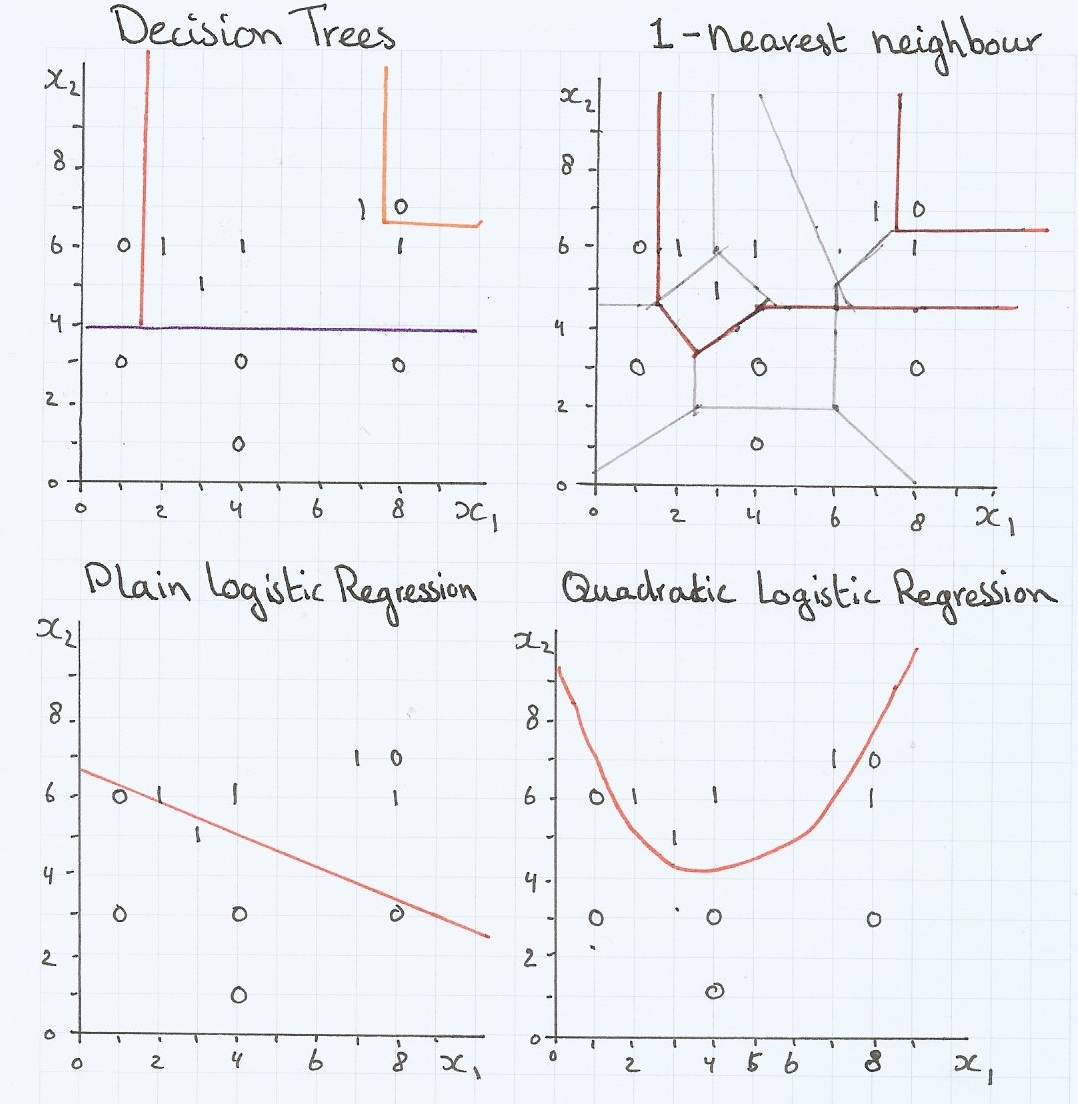
\includegraphics[width=\linewidth]{classification.JPG}
	\caption{Four kinds of classification}
	\label{fig:classification}
\end{figure}


\begin{figure}
	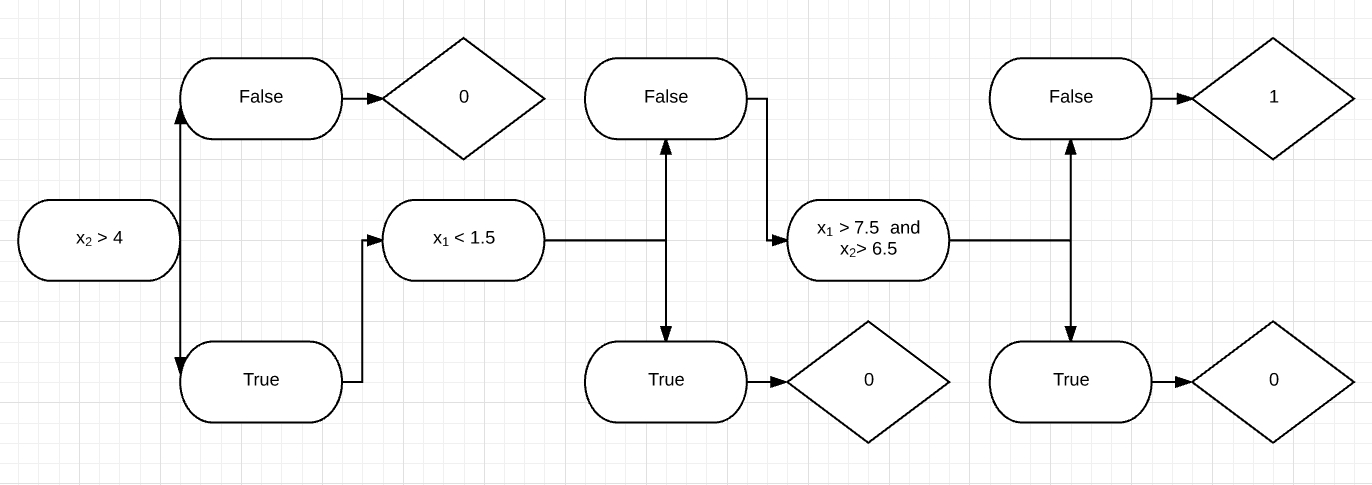
\includegraphics[width=\linewidth]{decisiontree.jpg}
	\caption{The decision tree used for classification}
	\label{fig:decistree}
\end{figure}

\pagebreak

\subsection{Do you intuitively think that one boundary is better than another?}
\textit{It may be possible to use such an intuition to invent method that uses
multiple learning algorithms and combine the results, using your intuition as a prior
probability. Explore this line of thought.}

I would like to start with excluding Plain Logistic Regression as there is no decision boundary found by this algorithm that will fit the data well, it is biased. The data asks for a non-linear decision boundary. Then, we have Decision Trees, 1-Nearest Neighbour and Quadratic Logistic Regression left. The decision boundaries found by the first two are very similar. They divide the plane in three areas, two of which are zeros and one for ones. It seems strange to have three areas for two values, so these methods are probably over-fitting. The last method is Quadratic Logistic Regression. This method doesn't fit the data perfectly, but only has one value that will be predicted wrong with my decision boundary, so it is neither over-fitting nor biased. Also, it divides the plane in two areas which fit the two outcomes. 

One thing that these three decision boundaries have in common is the fact that all inputs with $x_2 < 4$ have the value 0. We could combine the decision tree algorithm with quadratic logistic regression. we would first determine if $x_2 < 4$ is true, f it is we predict the example to belong to class 0; if it isn't we continue prediction using the boundary found by Quadratic Logistic Regression. The purpose of this is to prevent doing unnecessary computations, which could speed up predictions for big datasets considerably.

\section{Question 2} 
\textit{Manually calculate 1 iteration of k-means clustering for the 1-dimensional data below. Assume that there are 3 clusters and
initialize the means with 1, 3 and 8.  Calculate the cost before and after this step.
Data: 1, 2, 3, 3, 4, 5, 5, 7, 10, 11, 13, 14, 15, 17, 20, 21.}

The first step in the k-means clustering algorithm is to choose our initial clusters. In this case they are: $c_1 = 1$, $c_2 = 3$ and $c_3 = 8$. 
Then, we calculate the distance to each of these clusters for every input example and assign each to the nearest cluster, see table \ref{tab:firstit}.
The third step is to recalculate the mean value of each cluster, see equations (1) to (3). Finally, we would test if a stop condition has been met. In this case it has as we did our one iteration. 
Otherwise, we repeat the procedure of assigning clusters and recalculating means. 


\begin{align}
\mu_1 &= \frac{1 + 2}{2} &= 1.50\\
\mu_2 &= \frac{3+3+4+5+5}{5} &= 4.00\\
\mu_3 &= \frac{7+10+11+13+14+15+17+20+21}{9} &= 14.22
\end{align}

If we want to calculate the cost of the k-means function we calculate the average distance from each point to it's cluster. In order to do that we have to do one more cluster assignment for which we take $c_1 = 0.5$, $c_2 = 4$ and $c_3 = 14$ for convenience, see table \ref{tab:second}. We can then calculate the cost:

\begin{align*}
Cost_{before} &= \frac{(0+1)+(0+0+1+2+2) + (1+2+3+5+6+7+9+12+14)}{2+5+9}\\
 &= 4.0625\\
\\
Cost_{after} &= \frac{(0.5+0.5)+(1+1+0+1+1+3)+(4+3+1+0+1+3+6+8)}{2+6+8} \\
&= 2.125
\end{align*}

As we can see, even one iteration makes a profound difference in the cost. 

\section{Tables}

\begin{table}[h!]
\centering
\begin{tabular}{c c c c c}
& & Distance & & \\
 $x$ & $c_1$ & $c_2$ & $c_3$ & cluster\\
\hline
1 & 0 & 2 & 7 &$c_1$\\
2 & 1 & 1 & 6 & $c_1$\\
3 & 2 & 0 & 5 &$c_2$\\
3 & 2 & 0 & 5 & $c_2$\\
4 & 3 & 1  & 4 &$c_2$ \\
5 & 4 & 2 & 3 & $c_2$ \\
5 & 4 & 2 & 3 & $c_2$\\
7 & 6 & 4 & 1 & $c_3$\\
10 & 9  & 7 & 2 &$c_3$ \\
11 & 10  & 8 & 3 & $c_3$\\
13 & 12  & 10 & 5 & $c_3$ \\
14 & 13  & 11 & 6 & $c_3$\\
15 & 14  & 12 & 7 &$c_3$ \\
17 & 16  & 14 & 9 & $c_3$\\
20 & 19  & 17 & 12 &$c_3$ \\
22 & 21  & 19 & 14 & $c_3$ \\
\end{tabular}
\caption{The distance to each cluster and the nearest cluster  for every data point $x$.}
\label{tab:firstit}
\end{table}


\begin{table}[h!]
\centering
\begin{tabular}{c c c c c}
& & Distance & & \\
 $x$ & $c_1$ & $c_2$ & $c_3$ & cluster\\
\hline
1 & 0.5 & 3 & 13 &$c_1$\\
2 & 0.5 & 2 & 12 & $c_1$\\
3 & 1.5 & 1 & 11 &$c_2$\\
3 & 1.5 & 1 & 11 & $c_2$\\
4 & 2.5 & 0  & 10 &$c_2$ \\
5 & 3.5 & 1 & 9 & $c_2$ \\
5 & 3.5 & 1 & 9 & $c_2$\\
7 & 5.5 & 3 & 7 & $c_2$\\
10 & 8.5  & 6 & 4 &$c_3$ \\
11 & 9.5  & 7 & 3 & $c_3$\\
13 & 11.5  & 9 & 1 & $c_3$ \\
14 & 12.5  & 10 & 0 & $c_3$\\
15 & 13.5  & 11 & 1 &$c_3$ \\
17 & 15.5  & 13 & 3 & $c_3$\\
20 & 18.5  & 16 & 6 &$c_3$ \\
22 & 20.5  & 18 & 8 & $c_3$ \\
\end{tabular}
\caption{The distance to each cluster and the nearest cluster  for every data point $x$ after the first iteration.}
\label{tab:second}
\end{table}












\end{document}